\documentclass[herrin-thesis.tex]{subfiles}
\begin{document}

\chapter{Data Collection and Processing}
\label{ch:data}

\section{Signal Readout}
\begin{figure}
\centering
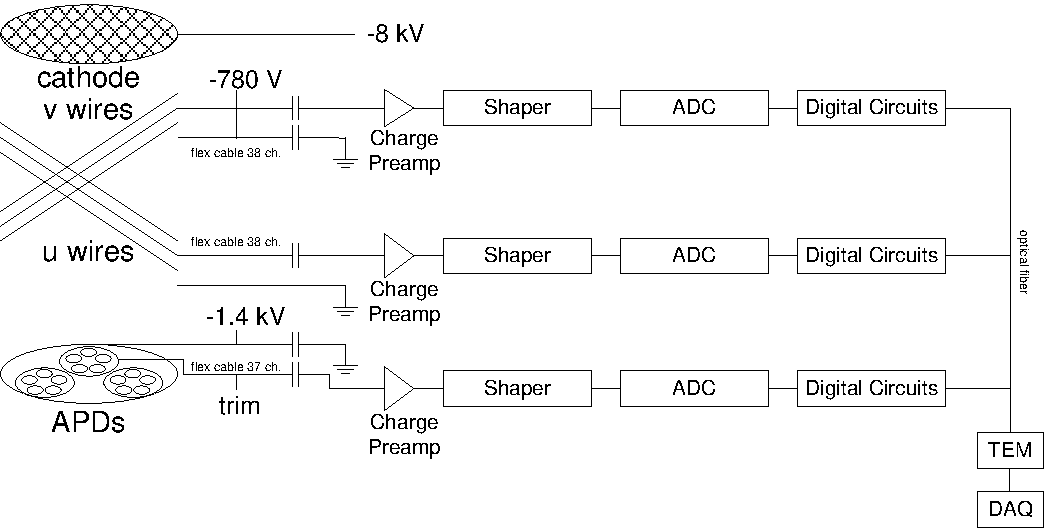
\includegraphics[width=\textwidth]{./figures/data_simplified_electronics.pdf}
\caption[The EXO-200 electronics]{A simplified schematic of the EXO-200 electronics. The ionization and scintillation signals are read out through long flex cables. The signals are shaped, digitized, and passed to the Trigger Event Module (TEM), which passes the data to the DAQ computers for recording when signals are detected.}
\label{fig:data_simplified_electronics}
\end{figure}

\begin{table}[tbp]
\centering
\caption[Electronic shaping times]{The shaping times for the signal readouts in EXO-200.}
\label{tab:data_shaping_times}
\begin{tabular}{l c c c c c}\toprule
				&						\multicolumn{5}{c}{Stage Type}										\\\cmidrule{2-6}
	Channel Type	&	\multicolumn{2}{c}{Integration (\si{\micro\s})}	&	\multicolumn{3}{c}{Differentiation (\si{\micro\s})}	\\\midrule
	APDs		&	3		&	3						&	10		&	10	&	300					\\
	\(u\) wires		&	1.5		&	1.5						&	40		&	40	&	60					\\
	\(v\) wires		&	3		&	3						&	10		&	10	&	60					\\\bottomrule
\end{tabular}
\end{table}

\Cref{fig:data_simplified_electronics} shows a simplified schematic for the EXO-200 electronics. The APD signals and the ionization inductions and collection signals are read out through long flex cables. The long cables separate the electronics from the TPC, removing the need for cryogenic and low-radioactivity components. After passing through a preamplifier, the signals are fed through shaping circuits and are then digitized at a rate of \SI{1}{\MHz}. The shaping circuits consist of two integrators followed by two differentiators and one final differentiator on the charge preamp. \Cref{tab:data_shaping_times} summarizes the time constants.

After digitization, the Trigger Event Module (TEM) monitors the signals to select interesting events. Due to the low radioactive backgrounds in EXO-200, and the relatively slow rate of \twonu, this trigger is extremely permissive. It is 100\% efficient at triggering on events that deposit more that \todo{Look up} in the liquid xenon. The average trigger rate during routine data taking is approximately \SI{8}{\mHz}. Additionally, the trigger is forced to fire every \SI{0.1}{\s} in order to ensure the DAQ system is correctly recording events and to provide a measurement of detector live time. When the trigger fires, the DAQ records a frame consisting of digitized waveforms for all channels \SI{\pm1024}{\micro\s} around the trigger time.

\section{Signal Reconstruction}
\subsection{Signal Finding}
Either scintillation or ionization signals may cause the trigger to fire. Since there is not a fixed time between the two types of signal, it is necessary to search for signals in the waveforms. This is done in a two stage process: first a matched filter technique searches for signals, and then a waveform unshaping technique refines the found signals. \Cref{fig:data_signal_finding} shows an example of this process.

\begin{figure}
	\centering
	\begin{subfigure}[t]{0.48\textwidth}
		\centering
		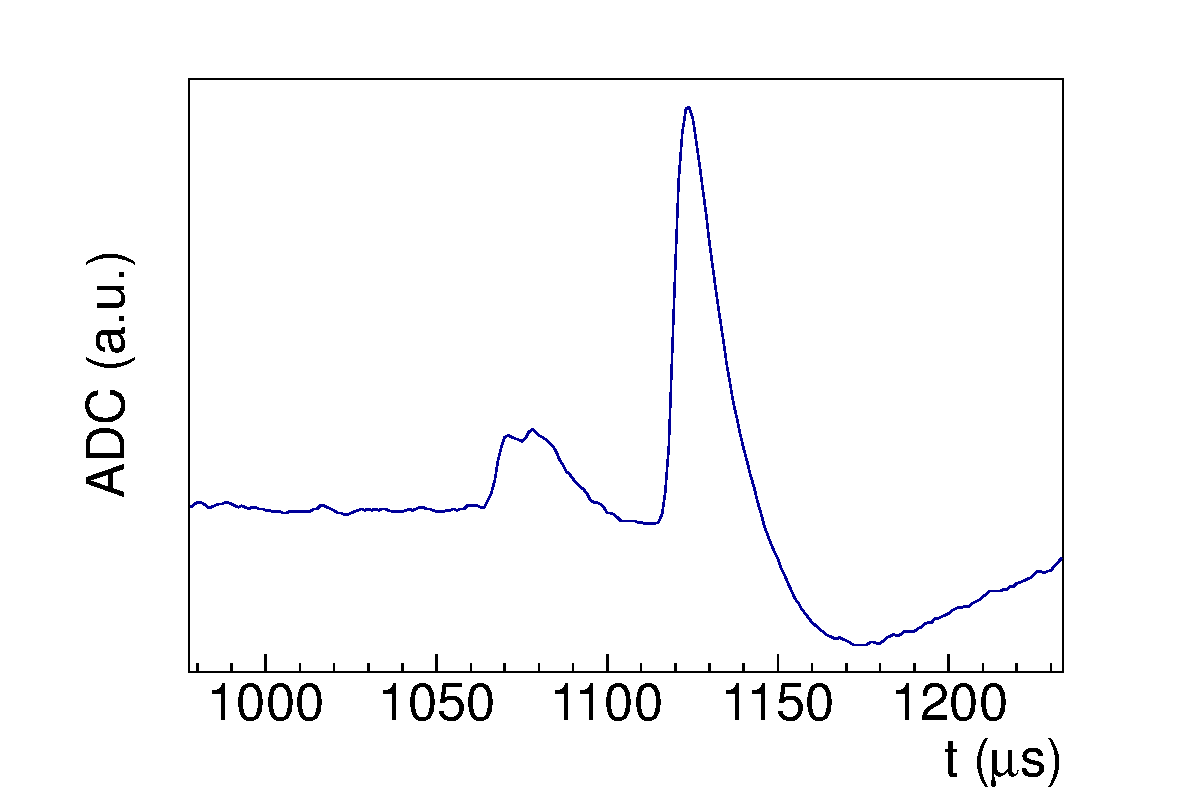
\includegraphics[width=\textwidth]{./plots/data_signal_finding_raw.pdf}
		\caption[Raw \(u\) wire waveform]{A raw \(u\) wire waveform showing two signals.}
		\label{fig:data_signal_finding_raw}
	\end{subfigure}\hfill%
	\begin{subfigure}[t]{0.48\textwidth}
		\centering
		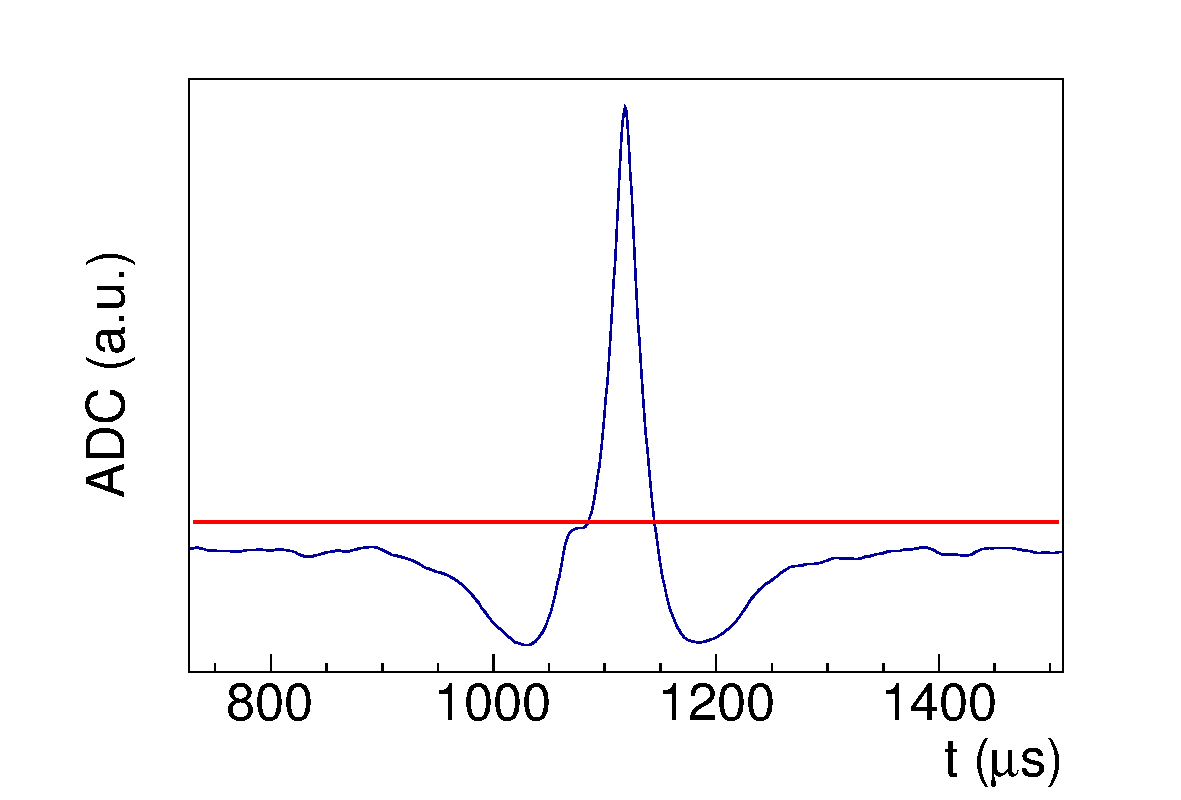
\includegraphics[width=\textwidth]{./plots/data_signal_finding_mf.pdf}
		\caption[Matched filter output]{The output of the matched filter with the threshold shown in red.}
		\label{fig:data_signal_finding_mf}
	\end{subfigure}
		\begin{subfigure}[t]{0.48\textwidth}
		\centering
		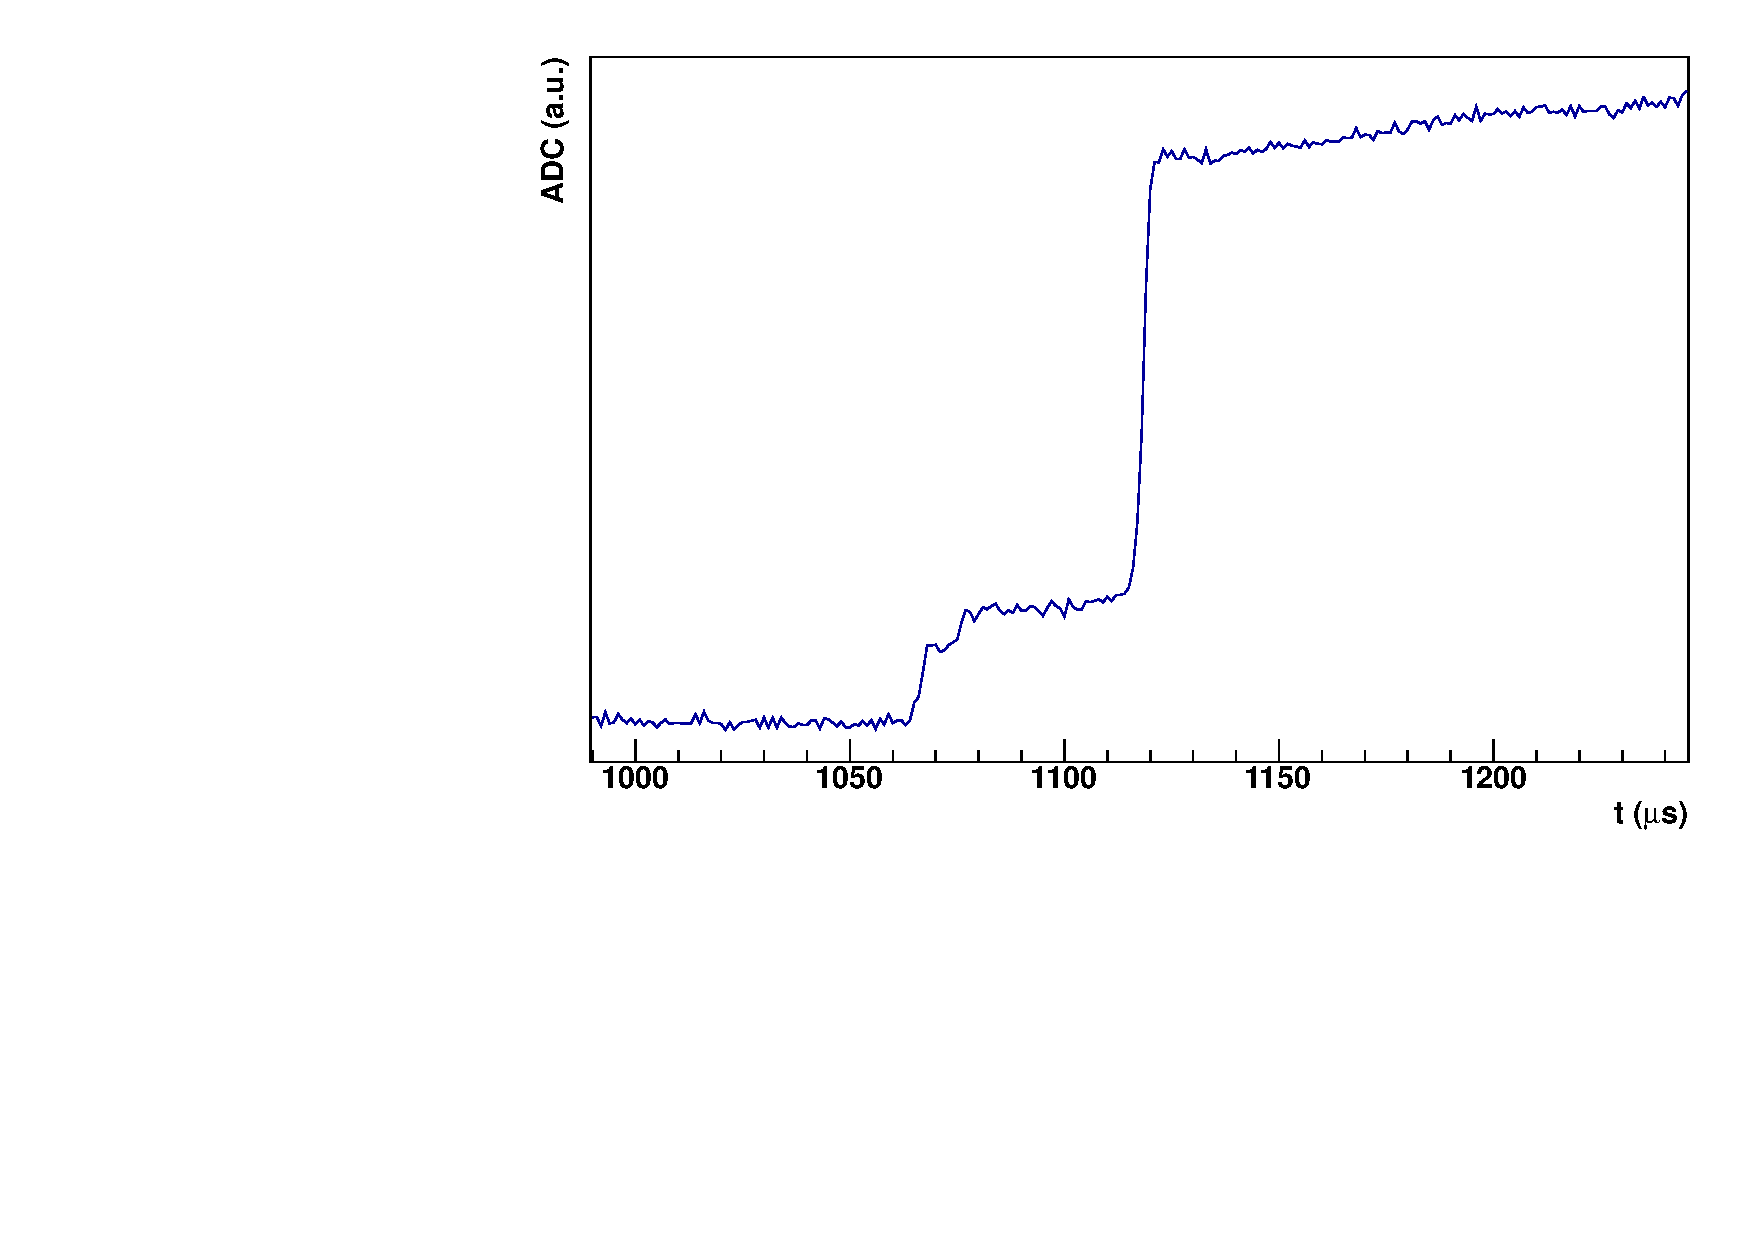
\includegraphics[width=\textwidth]{./plots/data_signal_finding_unshaped.pdf}
		\caption[Unshaped signals]{The `unshaped' signals.}
		\label{fig:data_signal_finding_unshaped}
	\end{subfigure}\hfill%
	\begin{subfigure}[t]{0.48\textwidth}
		\centering
		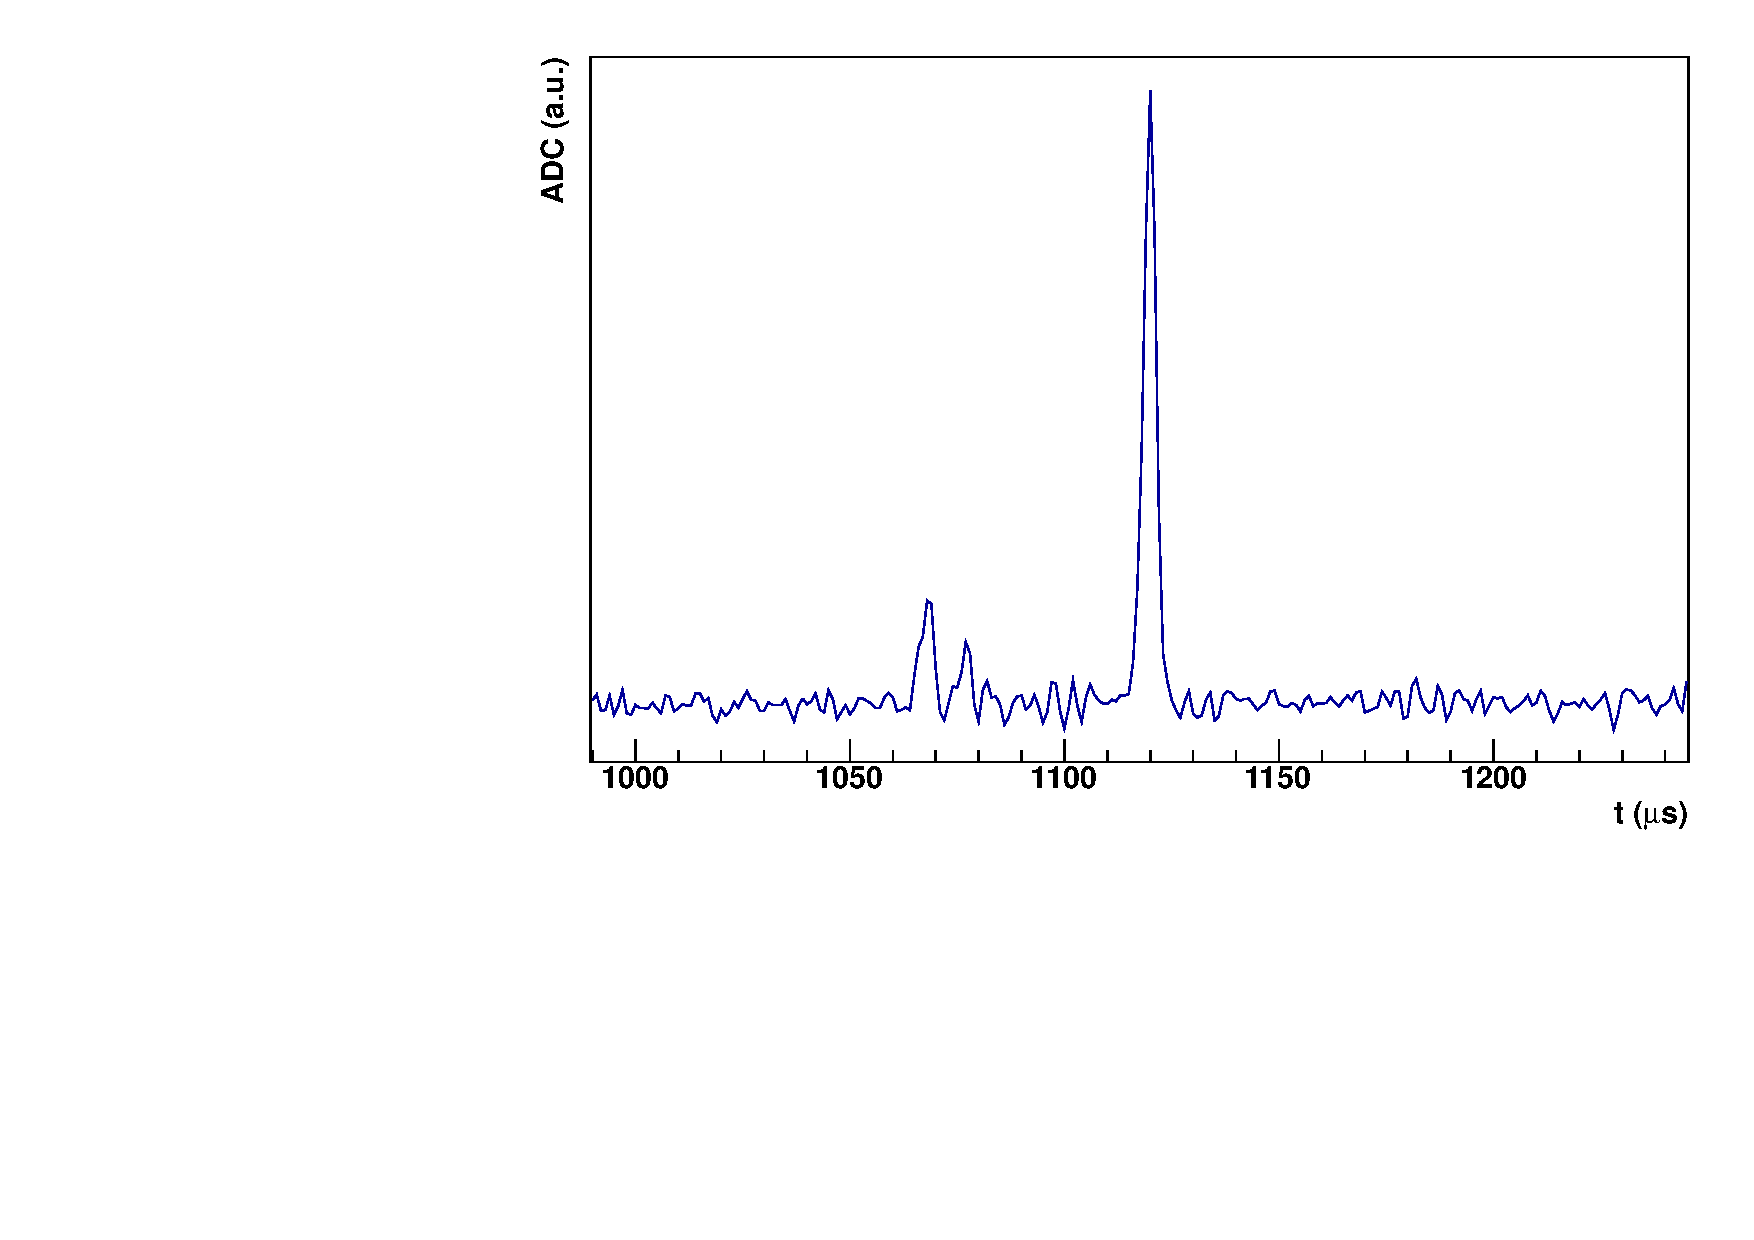
\includegraphics[width=\textwidth]{./plots/data_signal_finding_msf.pdf}
		\caption[Multiple signal finger output]{The output of a \SI{2}{\micro\s} triangular filter on the unshaped signals.}
		\label{fig:data_signal_finding_msf}
	\end{subfigure}
	\caption[The signal-finding process]{An example of finding signals on a \(u\) wire waveform.}
	\label{fig:data_signal_finding}
\end{figure}

The matched filter technique\cite{North:1963fk} convolves a time-reversed template signal with the waveform. Template signals are produced by passing a step function through the filters specified in \cref{tab:data_shaping_times}. This is done for individual channels for the \(u\) and \(v\) wires. For the APDs, the signals on the individual planes are summed and this technique is applied to these two sum signals. A threshold is determined by calculating the mean absolute deviation (MAD) of the waveform from its baseline. Parts of the waveform exceeding \((3\sqrt{\pi/2})\times\text{MAD}\) are excluded and the MAD is recalculated. A signal is found if the filter output exceeds 5 (4) times this final MAD for the wire (APD) signals. \Cref{fig:data_signal_finding_raw,fig:data_signal_finding_mf} show an example of this process.


\section{Corrections}
\subsection{Gain Corrections}
\subsection{Shielding Grid Corrections}
\subsection{Electron Lifetime Corrections}
\subsection{Light Collection Efficiency Corrections}

\section{Calibration}

\section{Data Quality Cuts}

\end{document}
